\documentclass[UTF8, a4paper]{ctexart}

\usepackage{geometry}
\usepackage{titlesec}
\usepackage{titletoc}
\usepackage{graphicx}
\usepackage{caption}
\usepackage{hyperref}
\usepackage{listings}
\usepackage{hyperref}
\usepackage{xcolor}
\usepackage{siunitx}
\usepackage{perpage}
\usepackage{amsmath}
\usepackage{fancyhdr}
\pagestyle{fancy}
\lfoot{}%这条语句可以让页码出现在下方

\lstset{
	numbers=left,
	numberstyle= \tiny,
	keywordstyle= \color{ blue!70},%设置关键字颜色
	commentstyle= \color{red!50!green!50!blue!50}, %设置注释颜色
	frame=lines, %设置边框, % 阴影效果
	rulesepcolor= \color{ red!20!green!20!blue!20} ,
	escapeinside=``, % 英文分号中可写入中文
	xleftmargin=2em, %距离左边界2em
	aboveskip=1em,
	framexleftmargin=2em,
	basicstyle=\ttfamily,
	columns=fullflexible,%可以自动换行
	linewidth=1\linewidth, %设置代码块与行同宽
	breaklines=true,%在单词边界处换行。
	showstringspaces=false, %去掉空格时产生的下划的空格标志, 设置为true则出现
	breakatwhitespace=ture,%可以在空格处换行
	escapechar=`%设置转义字符为反引号
}

\MakePerPage{footnote}

\geometry{a4paper, left = 2.7cm, right = 2.7cm, top = 2.54cm, bottom = 2.54cm}

\hypersetup{
	colorlinks=true,
	linkcolor=black
}

\captionsetup[figure]{skip=0pt}
\captionsetup[table]{skip=0pt}

\title{基于决策树模型和神经网络模型的降雨量问题研究}

\author{李沐阳 \and 钟绍恒 \and 易领程}

\begin {document}

\maketitle

% \tableofcontents

% \addcontentsline{tocloft}{section}{附录}

\section{摘要}

本文针对局部地区的降雨量与其它气象相关的因素进行了数学模型
的建立和求解的通用算法的设计,运用线性回归,障碍计数,时间序
列和神经网络等模型分别进行了尝试,最终发现决策树取得了较好的结果.

根据气象预测的要求,定义正确为与真实数据相差的绝对值小于$10$\si{\milli\meter}.我们
首先针对与降水量关联度最大的水平面气压\footnote{以下简称为``气压``} 和气
温等条件,将数据按照$30$天为一组进行平均处理整理后,根据气象学上的基
本原理,运用线性回归模型拟合真实数据,完成了该简单模型的求解,取得了
正确率$53 \%$和绝对平均误差$11$mm的良好的预测效果,在这里同时使用了最
小二乘法进行拟合,均能够取得很好的效果.在此时还尝试了障碍计
数模型来应对未降雨的情况,但尝试后发现准确率极低,只有$6\%$左右,整
理数据后分析得到数据的趋势具有连续变量的特征,趋势上大致更加符合回归模型这一类.

随后扩大研究的范围,添加了云层覆盖,湿度,风速为新的自变量,由于此时线
性回归在多个自变量的的相互影响下适应性较差,转变模型,根据深度学习的基本
原理和神经网络中防止过拟合的技术,运用了神经网络回归模型进行拟合,在仅
使用$5$个神经层,共$200$多个神经元的情况下取得了绝对平均误差仅
为$9$\si{\milli\meter}的优异结果 .同时,我们也展开了遗传算法训练网络的尝试,在有$4$层,分别
为$5,20,20,1$个神经元的网络中,发现每个个体网络无论输入,输出值均为$26$\si{\milli\meter}上下,
同时,各个个体逐渐趋同演化,丧失了物种多样性,经过$100$代后,每个个体的适
应度已相同,很难进化,最后无奈放弃此方法,猜测是遗传算法并不适合此种情况神经
网络的训练,但依旧提供了一种解决问题的新思路.

在数据具有明显季节性质,且相邻的日期可能相互影响的情况下,我们也
对时间序列模型进行了一定的尝试和研究,最后得到的效果也不如神经网
络回归模型,原因可能是相互影响因素已经体现在了自变量中.经过进一步
的分析,尽管数据间并非存在明显的非线性关系,但是由于数据具有取值
范围相对局限的特点,我们尝试了决策树模型,最终得到了满意
的结果,绝对平均误差降到了$2.6$mm,正确率飙升到$88\%$左右.尝试和分
析过后,最后认为该决策树模型更加准确.

该模型具有预测率较高,和可以轻易扩展到新的自变量的优点.生成该模型
的方法可以轻易地被用于生成任何局部降雨模型,非常简单易行.在考虑到气
象的周期性而忽略人为影响的情况下,本模型具有较为准确的预测能力.
同时,实际上,降雨量的影响因素更加复杂,采用该模型时可以增加自变量
的数量,进一步提高模型的准确度,具有一定的现实指导意义.

\null\vfill % 这里的\null可以使当前行为空,\vfill则填充所有垂直空间
\begin{flushleft}
	\begin{tabular}{
		>{\centering}p{0.1\textwidth}
		>{\centering}p{0.25\textwidth}
		>{\centering}p{0.2\textwidth}
		>{\centering}p{0.15\textwidth}
		>{\centering}p{0.15\textwidth}}
		\textbf{关键词}: & 神经网络回归模型 & 线性回归模型 & 遗传算法 & 决策树模型
	\end{tabular}
\end{flushleft}

\newpage

\section{问题重述}

在过去的几十年中,随着各行各业的迅速发展,气象对于人类生产生活的影响日益
显著,对于气象预测的精确程度需要愈来愈高,降雨作为人们出行和农业生产的客
观需要是非常关键的一部分.在当今时代,由于人类活动的影响日益增大和气象全
球性变化的影响下,气象的预测越来越有必要与时俱进,因地制宜的适应局部气候的变化.

请以气温、降水、气压、云层覆盖、风速、湿度为自变量,预测气象的降雨量.

\section{模型假设和符号说明}

\subsection{模型假设}
该模型假设气象活动完全是周期性的,不考虑气候的逐渐变化,也不考虑人为因素的气候的干扰.

同时,假设在自然条件下,降水量只与气温、降水量、气压、云层覆盖、风速、湿度有关系.

\subsection{符号说明}

为了方便表述,我们将符号简写为$p,r,t,f,h,c$,同时,为了简化单位,我们规定了每个符号的默认单位.

以下若无特殊说明,则默认单位为下表所示的单位.

\begin{table}[h!]
	\centering
	\caption{符号说明}
	\begin{tabular}{p{6em}p{6em}l}
		\hline
		符号  & 说明   & 单位                          \\
		\hline
		$r$ & 降雨量  & \si{\milli\meter}           \\
		$t$ & 温度   & $0.1$\si{\degreeCelsius}    \\
		$f$ & 风速   & $0.1$\si{\meter\per\second} \\
		$h$ & 湿度   & $0.1\%$                     \\
		$c$ & 云层覆盖 & \si{octas}                  \\
		$p$ & 气压   & $0.1$\si{h\pascal}          \\
		\hline
	\end{tabular}
\end{table}

\section{模型建立与求解}

\subsection{获取数据}

本文主要数据从欧洲气象网站\footnote{见附录~\textcolor{red}{\ref{data}}.} 关
于$11$号(\verb+STAID000011+)气象站(一个奥地利气象站)中获取,考虑到尽可能减少人类
活动的影响,本文主要取用了该奥地利气象站附近地区从$1877$年到$2000$的$r,t,f,h,c,p$,
为了简单起见,并没有选择辐射等可能影响因素相对较小的变量.


\subsection{数据预处理}

获取完数据之后,按照$30$天为一组进行平均\footnote{遗传算法中采用$1$个月为$1$组进行平均.},整理
完毕后,画出各个自变量的图像如下:
\begin{figure}[h!]
	\centering
	\begin{minipage}[h!]{0.4\textwidth}
		\centering
		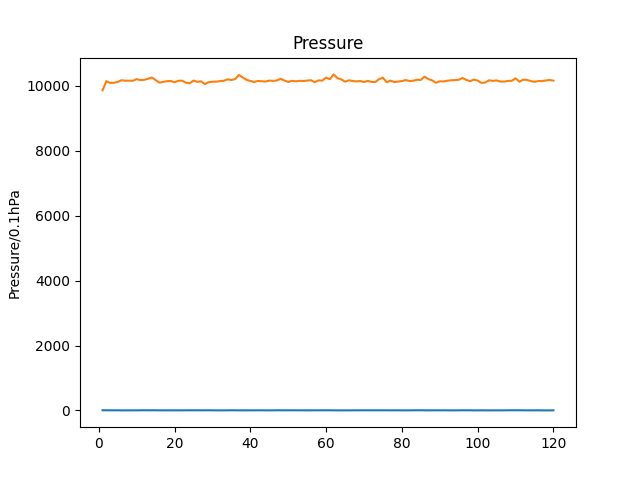
\includegraphics[scale=0.3]{../src/prepare_data/pp.png}
		\caption{气压覆盖关于时间的折线图}
	\end{minipage}
	\qquad
	\begin{minipage}[h!]{0.4\textwidth}
		\centering
		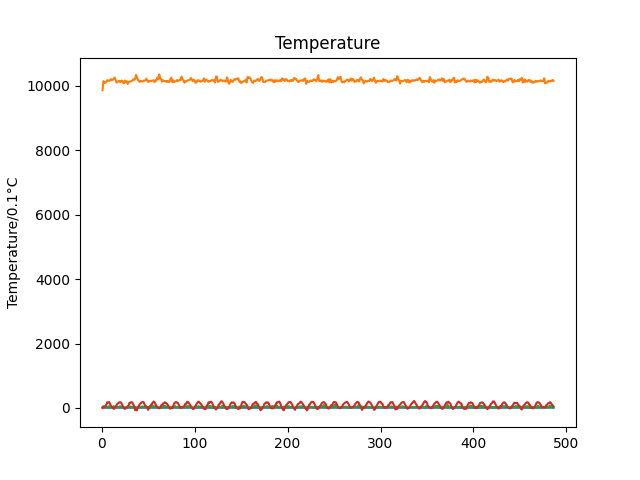
\includegraphics[scale=0.3]{../src/prepare_data/tg.png}
		\caption{气温关于时间的折线图}
	\end{minipage}
\end{figure}

\begin{figure}[h!]
	\centering
	\begin{minipage}[h!]{0.4\textwidth}
		\centering
		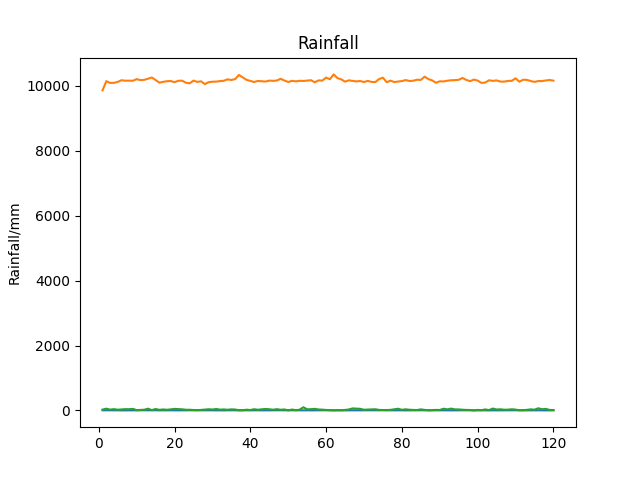
\includegraphics[scale=0.3]{../src/prepare_data/rr.png}
		\caption{降水量关于时间的折线图}
	\end{minipage}
	\begin{minipage}[h!]{0.4\textwidth}
		\centering
		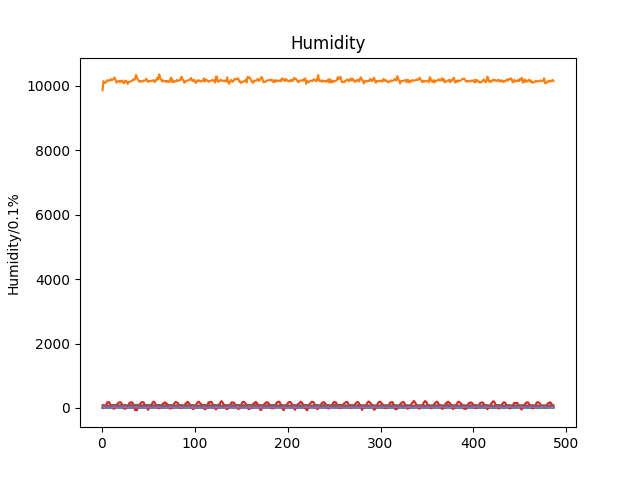
\includegraphics[scale=0.3]{../src/prepare_data/hu.png}
		\caption{湿度关于时间的折线图}
	\end{minipage}
\end{figure}

\begin{figure}[h!]
	\centering
	\begin{minipage}[h!]{0.4\textwidth}
		\centering
		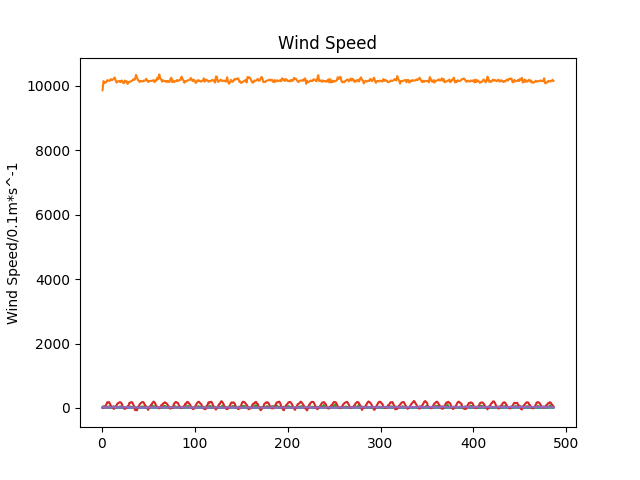
\includegraphics[scale=0.3]{../src/prepare_data/fg.png}
		\caption{风速关于时间的折线图}
	\end{minipage}
	\begin{minipage}[h!]{0.4\textwidth}
		\centering
		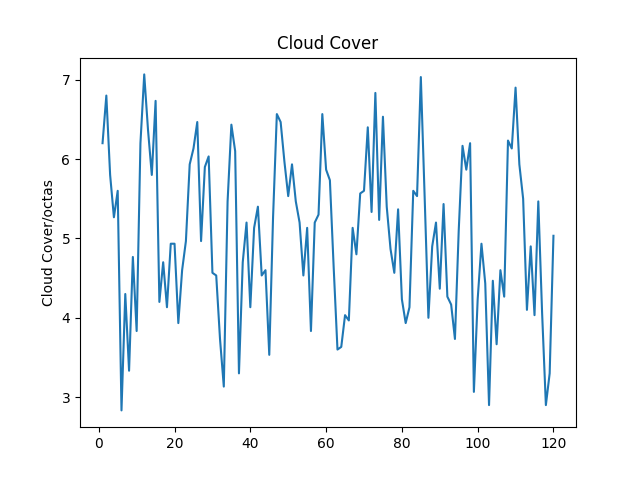
\includegraphics[scale=0.3]{../src/prepare_data/cc.png}
		\caption{云层覆盖关于时间的折线图}
	\end{minipage}
\end{figure}

\subsection{拟合模型}

\subsubsection{线性回归模型}

简单研究,发现$r,t,p$呈一定的周期关系,且在周期内大致成趋势一致,猜测之间很可能呈线性关系,建
立线性回归模型 $r=at+bp$,使用最小二乘法让程序生成对应的模型\footnote{该程序见附
	录~\textcolor{red}{ \ref{liner_program}}.},从而拟合最多的数据,得到结果为
$$r=0.1168736t+0.00188574p$$画出拟合图像与真实图像如图~\textcolor{red}{\ref{pic7}}.

\begin{figure}[h!]
	\centering
	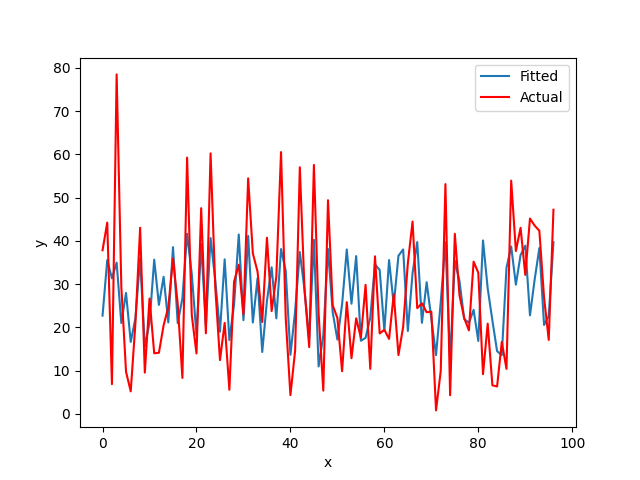
\includegraphics[scale=0.3]{fit1.png}
	\caption{拟合降水量和真实降水量的折线统计图\label{pic7}}

\end{figure}
可以看到数据趋势基本相符,但是相比于实际数据没有那么极端,此时正
确率达到$52\%$左右,绝对平均误差达到$10$mm,考虑到模型的吻合性其
实不弱,应当是气象影响因素比较复杂的缘故,于是寻找新的自变量来考
虑的更加全面.经过一番对气象基本的研究,我们添加了$f,c,h$这三
个比较相关的变量.

根据对数据关系的分析,发现此时已经有部分数据并不是时刻满足线性
关系,但总体上还比较吻合,尝试继续用线性回归模型刻画,使用最
小二乘法,得到模型为:
\begin{align}
	\notag
	r & =6.264621458073717c+0.23936949821555784h+0.18358187666124123t \\
	\notag
	  & \qquad -0.004092803931093655p+0.23939598907957882f
\end{align}
该模型的描述能力确实有一定程度上的提高,绝对
平均误差保持在$10$mm,但是正确率达到了$64\%$左右,以下
是5个自变量时的拟合图像:

\begin{figure}[h!]
	\centering
	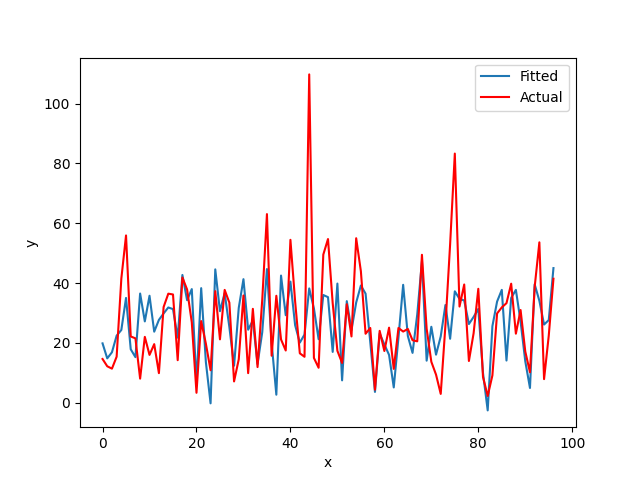
\includegraphics[scale=0.3]{fit2.png}
	\caption{拟合降水量和真实降水量的折线统计图}
\end{figure}

观察后可以发现该模型更加准确了,但是离设想中还有一定的距离.考虑
到数据波动较大,因此得出:回归模型适合描述该问题的模型.但线性回
归模型局限性略大,可能在变量之间的相互影响的作用下导致某些关系并非线性.

\subsubsection{障碍计数模型}

尝试障碍计数模型,仅得到了$6\%$的准确率,因此障碍计数模型并不适合解决
该问题.

\subsubsection{神经网络}

经过最初的尝试后,首先确定了$5$个神经元层,分别是$64$,$64$,$64$,$64$,$1$,
若神经元数量再多过拟合的风险很大,若过少也很容易造成对训练数据和测试数
据正确率都降低的情况,这样的数据是比较合理的.训练方法是传统的梯度下降反向传播算法,在对神经网络激活函数的选
择中,我们最初选择了\verb+sigmoid+,后来经过讨论,认为该二分类型激活函数不适
合该背景,改为了\verb+leaky relu+函数,大大提升了最初的训练速度.\footnote{该神经网络训
	练程序见附录~\textcolor{red}{\ref{net_program}}.}

经过初步调整参数,将训练次数定为比较合适的$300$次,$200\sim300$次均有不错
的效果,但此时过拟合已经十分严重,在训练数据上达到了甚至达到了$100\%$,然
而在测试数据上只有糟糕的$60\%$,经过一系列的尝试,我们使用了\verb+L2+正则化和\verb+dropout+
的方式,再加上早停的策略(采用的是比较宽松的早停策略,并且会记录下训练中的最
佳权值,训练一般进行$100$多次就会被早停),成功的把训练数据和测试数据拉到一个
水平线上,由于该模型需要用几个$64\times64$的矩阵描述,过于占篇幅,故在此处不给出.

此时,模型已经达到了一个比较优秀的地步,正确率达到了$74\%$左右,绝对平均误差降
到了$8$\si{\milli\meter}左右,绘制一下拟合图像:

\begin{figure}[h!]
	\centering
	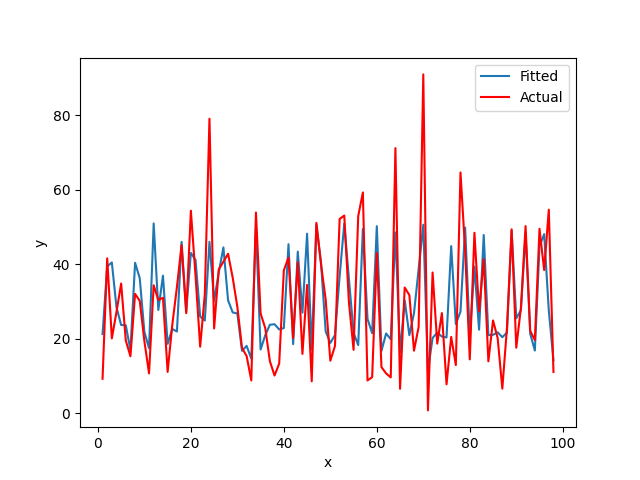
\includegraphics[scale=0.3]{success.png}
	\caption{拟合降水量和真实降水量的折线统计图}
\end{figure}

非常明显,相比与之前的线性回归模型,神经网络回归模型的拟合准确度明
显大大增强,但是对于某些特别极端的值似乎依旧有一些缺失,不过总体
拟合的还算准确.

猜测用遗传算法训练网络会有更好的结果,我们也展开了尝试,但经过切换各种激活函数
和初始化方法,发现网络得到的值方差较小,有靠拢趋势,在经过$1000$代后,所有的个体
的适应度都逐步收敛到一个值上,同时所有个体的策略都是无论输入,输出都是相
同的值,并不符合现实情况,对现实指导的意义不大.针对这种情况,我们猜想是因为
遗传算法对局部搜索能力不够强大,导致了网络的学习效率低下.同时我们采用的算法
也不太适合用于神经网络模型训练,我们只将其作为一种特殊的模型进行尝试,提供新的思路.

\subsubsection{决策树模型}

下一步就是对模型类型进行进一步的尝试,我们首先对与神经网络模型在处理关系
不明显数据方面同样显著的决策树模型,进行了检验,从理论上来看,数据间并非存
在明显的非线性关系,这样的问题应当不太适合使用决策树模型刻画,但是对于降水
量这样取值范围较为固定和小的特殊问题,用决策树模型可能也会有特殊的好效果,
决策树模型的代码因为与线性前两个模型相似度很高,在此处不贴出.决策树模
型的拟合图像如图~\textcolor{red}{\ref{pic10}}.

\begin{figure}[h!]
	\centering
	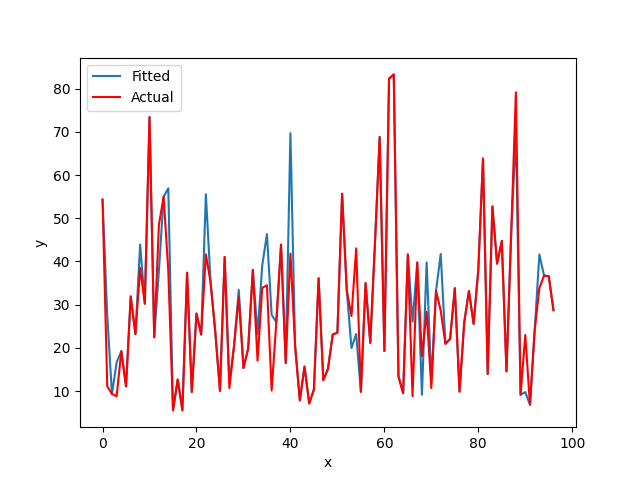
\includegraphics[scale=0.3]{very_success.png}
	\caption{拟合降水量和真实降水量的折线统计图}\label{pic10}
\end{figure}

拟合程度很高的图像.绝对平均误差从$8.9$\si{\milli\meter}骤降到$2.7$\si{\milli\meter},而正确率飙升到$88\%$,结果较好.

由于我们的数据范围较大,决策树模型的训练算法会尽量在较大尺度上寻找数据的普遍规律,具有一定的准确度,决策树模型通过,对于给定数据的每一个取值都产生一个相应的分支来拟合数据,虽然存在属性的交叉,但是数据范围还是比较大

仔细分析,可以得知也许是因为欧洲气象较为平均,没那么极端,决策树模型虽然尝试在较大的尺度上寻找数据普遍的分类依据,究其
本质还是一种另类的分类讨论,若是在气象多变的广东地区,数据量相同的情况下,效果也许反而不如神经网
络模型.神经网络模型和线性回归模型从本质上探索他们之间的数量关系,但决策树模型
只是分类讨论罢了,对于出现次数少的预测能力不足,但是实践证明,也是一种非常切实可行的方案了.
\footnote{见附录~\textcolor{red}{\ref{tree_result}}.}


\section{模型的优缺点与改进方法}

\subsection{线性回归模型}
基于线性回归模型在仅研究几个变量的时候准确度和神经网络回
归模型相差无几,具有操作十分简单,预测能力也并不算很弱
的特点,改进方法也许可以采用并非完全线性的回归模型,对
于某些变量进行更加具体的分析,采用其他的基本函数进行描述效果可能会好一点

\subsection{神经网络回归模型}
基于神经网络的模型具有普适性更加强的特点,在降雨量受到如此
多方面的影响的情况下对其中的几个关键变量进行研究能达到还不
错的效果,实践起来也不算特别麻烦.

该方法可以利用神经网络强大的调整和适应能力用来研究各个地区的局部降雨量.
不足之处在于,若是把时间范围拉得很大,会导致模型由于气候变化和人类活动导致不
准确性增加,而且模型也并没有针对季节等进行描述.

可以从两方面考虑增强方法,一是结合一定的时间序列模型来解决气候变化和人类活动
的问题,因为这两个因素也是按照一定的规律变化的,神经网络可以学
习出其中的趋势;二是考虑季节性的特点,一定程度上可以使用有季节性
的时间序列模型来缓解.但还有一种思路就是添加更多的自变量来间接
反应季节的影响,因为气象总体是呈周期性的,例如可以添加风向作为
自变量,来间接的反映季风,进而反映出季节的变化,感觉这种思路可
能会好一点.

\subsection{决策树模型}
由于决策树模型具有可以随意调整叶子节点和非叶子节点的分界点,从而使数
据尽可能的良好匹配所有的数据的特性和天气取值范围并不是很大的特点,
使得它对于气候这种并非不具有显著函数关系的问题拟合程度非常高,几乎
可以说是十分精确的预测了.

另一方面,对于极端情况的预测效果一定是很差的,因为数据被设计的
尽量靠近正常的数据了,就会使得偏离不常出现的值.

但是,若是我们把前两个模型综合起来看,使用线性回归模型和神经网络
回归模型生成极端数据,再交由决策树模型拟合,就可以在一定程度上缓解
这个问题,三个模型可以相辅相成,决策树模型也可以反过来帮助神经网络
模型缓解过拟合的问题.

% \section{参考文献}

\appendix
\setcounter{secnumdepth}{-2}
\section{附录}

\setcounter{secnumdepth}{3}
\subsection{源代码}

\href{https://github.com/limuy2022/math_model}{完整代码和数据}

\subsection{数据来源}\label{data}

\href{https://www.ecad.eu/}{European Climate Assessment  Dataset}

\subsection{线性回归模型核心代码}\label{liner_program}

\begin{lstlisting}
	data = pd.read_csv('merged_data_file.csv')
	y_data = pd.read_csv("../tmprr.csv")
	y_data = y_data['RR'].values
	data_numpy = data.to_numpy()
	print(data_numpy)
	data_without_first_column = data_numpy[:, 1:]
	print(data_without_first_column)
	# 创建线性回归模型
	model = sm.OLS(y_data, data_without_first_column)
	res = model.fit()
	
	print("train rate:", get_rate1(res, data_without_first_column, y_data))
	print("train rate2:", get_rate2(res, data_without_first_column, y_data))
	test_data_num = int(len(data_without_first_column) * 0.2)
	test_idx = np.random.choice(len(data_without_first_column), test_data_num, replace=False)
	test_x = data_without_first_column[test_idx]
	test_y = y_data[test_idx]
	print("test rate:", get_rate1(res, test_x, test_y))
	print("test rate2:", get_rate2(res, test_x, test_y))
	print(res.params, )
	draw(range(len(test_x)), test_y, res.predict(test_x))
\end{lstlisting}

\subsection{神经网络回归模型核心代码}\label{net_program}
\begin{lstlisting}
	scaler = StandardScaler()
	X_scaled = scaler.fit_transform(data_without_first_column)
	y_scaled = scaler.fit_transform(y_data.reshape(-1, 1))
	X_train, X_test, y_train, y_test = train_test_split(X_scaled, y_scaled, test_size=0.2, random_state=42)
	early_stopping = EarlyStopping(monitor='val_loss', patience=10, restore_best_weights=True)
	model = tensorflow.keras.models.Sequential()
	model.add(Dense(64, activation='leaky_relu'))
	model.add(Dense(64, activation='leaky_relu', kernel_regularizer=l2(0.01)))
	model.add(Dropout(0.5))
	model.add(Dense(64, activation='leaky_relu', kernel_regularizer=l2(0.02)))
	model.add(Dropout(0.5))
	model.add(Dense(64, activation='leaky_relu', kernel_regularizer=l2(0.02)))
	model.add(Dropout(0.5))
	# model.add(Dense(64, activation='relu'))
	model.add(Dense(64, activation='leaky_relu'))
	model.add(Dense(1))
	
	model.compile(loss='mean_squared_error', optimizer='adam')
	model.fit(X_train, y_train, epochs=300, batch_size=32, validation_data=(X_test, y_test), callbacks=[early_stopping])
\end{lstlisting}

\subsection{决策树模型结果}\label{tree_result}
\begin{lstlisting}
|--- tg <= 125.83
|   |--- pp <= 10184.67
|   |   |--- fg <= 33.62
|   |   |   |--- tg <= 90.17
|   |   |   |   |--- cc <= 6.15
|   |   |   |   |   |--- pp <= 10119.95
|   |   |   |   |   |   |--- fg <= 23.30
|   |   |   |   |   |   |   |--- cc <= 5.27
|   |   |   |   |   |   |   |   |--- pp <= 10094.93
|   |   |   |   |   |   |   |   |   |--- value: [9.43]
|   |   |   |   |   |   |   |   |--- pp >  10094.93
|   |   |   |   |   |   |   |   |   |--- tg <= 47.38
|   |   |   |   |   |   |   |   |   |   |--- value: [22.63]
|   |   |   |   |   |   |   |   |   |--- tg >  47.38
|   |   |   |   |   |   |   |   |   |   |--- pp <= 10101.75
|   |   |   |   |   |   |   |   |   |   |   |--- value: [18.43]
|   |   |   |   |   |   |   |   |   |   |--- pp >  10101.75
|   |   |   |   |   |   |   |   |   |   |   |--- truncated branch of depth 2
|   |   |   |   |   |   |   |--- cc >  5.27
|   |   |   |   |   |   |   |   |--- hu <= 79.85
|   |   |   |   |   |   |   |   |   |--- value: [32.23]
|   |   |   |   |   |   |   |   |--- hu >  79.85
|   |   |   |   |   |   |   |   |   |--- hu <= 85.78
|   |   |   |   |   |   |   |   |   |   |--- tg <= 37.20
|   |   |   |   |   |   |   |   |   |   |   |--- value: [22.50]
|   |   |   |   |   |   |   |   |   |   |--- tg >  37.20
|   |   |   |   |   |   |   |   |   |   |   |--- truncated branch of depth 2
|   |   |   |   |   |   |   |   |   |--- hu >  85.78
|   |   |   |   |   |   |   |   |   |   |--- fg <= 16.05
|   |   |   |   |   |   |   |   |   |   |   |--- value: [22.17]
|   |   |   |   |   |   |   |   |   |   |--- fg >  16.05
|   |   |   |   |   |   |   |   |   |   |   |--- value: [20.67]
|   |   |   |   |   |   |--- fg >  23.30
|   |   |   |   |   |   |   |--- pp <= 10094.75
|   |   |   |   |   |   |   |   |--- cc <= 5.50
|   |   |   |   |   |   |   |   |   |--- value: [15.57]
|   |   |   |   |   |   |   |   |--- cc >  5.50
|   |   |   |   |   |   |   |   |   |--- tg <= 17.10
|   |   |   |   |   |   |   |   |   |   |--- value: [25.47]
|   |   |   |   |   |   |   |   |   |--- tg >  17.10
|   |   |   |   |   |   |   |   |   |   |--- value: [26.67]
|   |   |   |   |   |   |   |--- pp >  10094.75
|   |   |   |   |   |   |   |   |--- fg <= 30.63
|   |   |   |   |   |   |   |   |   |--- cc <= 5.97
|   |   |   |   |   |   |   |   |   |   |--- fg <= 29.10
|   |   |   |   |   |   |   |   |   |   |   |--- truncated branch of depth 3
|   |   |   |   |   |   |   |   |   |   |--- fg >  29.10
|   |   |   |   |   |   |   |   |   |   |   |--- truncated branch of depth 2
|   |   |   |   |   |   |   |   |   |--- cc >  5.97
|   |   |   |   |   |   |   |   |   |   |--- value: [37.77]
|   |   |   |   |   |   |   |   |--- fg >  30.63
|   |   |   |   |   |   |   |   |   |--- value: [41.03]
|   |   |   |   |   |--- pp >  10119.95
|   |   |   |   |   |   |--- pp <= 10166.18
|   |   |   |   |   |   |   |--- pp <= 10132.92
|   |   |   |   |   |   |   |   |--- fg <= 17.53
|   |   |   |   |   |   |   |   |   |--- tg <= -49.82
|   |   |   |   |   |   |   |   |   |   |--- value: [3.30]
|   |   |   |   |   |   |   |   |   |--- tg >  -49.82
|   |   |   |   |   |   |   |   |   |   |--- cc <= 5.67
|   |   |   |   |   |   |   |   |   |   |   |--- value: [5.37]
|   |   |   |   |   |   |   |   |   |   |--- cc >  5.67
|   |   |   |   |   |   |   |   |   |   |   |--- value: [6.33]
|   |   |   |   |   |   |   |   |--- fg >  17.53
|   |   |   |   |   |   |   |   |   |--- tg <= 46.23
|   |   |   |   |   |   |   |   |   |   |--- cc <= 5.37
|   |   |   |   |   |   |   |   |   |   |   |--- value: [33.43]
|   |   |   |   |   |   |   |   |   |   |--- cc >  5.37
|   |   |   |   |   |   |   |   |   |   |   |--- value: [25.73]
|   |   |   |   |   |   |   |   |   |--- tg >  46.23
|   |   |   |   |   |   |   |   |   |   |--- tg <= 85.38
|   |   |   |   |   |   |   |   |   |   |   |--- truncated branch of depth 3
|   |   |   |   |   |   |   |   |   |   |--- tg >  85.38
|   |   |   |   |   |   |   |   |   |   |   |--- truncated branch of depth 2
|   |   |   |   |   |   |   |--- pp >  10132.92
|   |   |   |   |   |   |   |   |--- hu <= 74.67
|   |   |   |   |   |   |   |   |   |--- value: [40.23]
|   |   |   |   |   |   |   |   |--- hu >  74.67
|   |   |   |   |   |   |   |   |   |--- tg <= 19.92
|   |   |   |   |   |   |   |   |   |   |--- cc <= 4.92
|   |   |   |   |   |   |   |   |   |   |   |--- truncated branch of depth 2
|   |   |   |   |   |   |   |   |   |   |--- cc >  4.92
|   |   |   |   |   |   |   |   |   |   |   |--- truncated branch of depth 9
|   |   |   |   |   |   |   |   |   |--- tg >  19.92
|   |   |   |   |   |   |   |   |   |   |--- tg <= 57.80
|   |   |   |   |   |   |   |   |   |   |   |--- truncated branch of depth 5
|   |   |   |   |   |   |   |   |   |   |--- tg >  57.80
|   |   |   |   |   |   |   |   |   |   |   |--- truncated branch of depth 6
|   |   |   |   |   |   |--- pp >  10166.18
|   |   |   |   |   |   |   |--- fg <= 27.58
|   |   |   |   |   |   |   |   |--- cc <= 5.25
|   |   |   |   |   |   |   |   |   |--- hu <= 88.58
|   |   |   |   |   |   |   |   |   |   |--- cc <= 4.77
|   |   |   |   |   |   |   |   |   |   |   |--- truncated branch of depth 3
|   |   |   |   |   |   |   |   |   |   |--- cc >  4.77
|   |   |   |   |   |   |   |   |   |   |   |--- value: [11.50]
|   |   |   |   |   |   |   |   |   |--- hu >  88.58
|   |   |   |   |   |   |   |   |   |   |--- value: [2.93]
|   |   |   |   |   |   |   |   |--- cc >  5.25
|   |   |   |   |   |   |   |   |   |--- pp <= 10172.18
|   |   |   |   |   |   |   |   |   |   |--- hu <= 87.33
|   |   |   |   |   |   |   |   |   |   |   |--- value: [13.07]
|   |   |   |   |   |   |   |   |   |   |--- hu >  87.33
|   |   |   |   |   |   |   |   |   |   |   |--- value: [9.80]
|   |   |   |   |   |   |   |   |   |--- pp >  10172.18
|   |   |   |   |   |   |   |   |   |   |--- cc <= 5.67
|   |   |   |   |   |   |   |   |   |   |   |--- value: [19.30]
|   |   |   |   |   |   |   |   |   |   |--- cc >  5.67
|   |   |   |   |   |   |   |   |   |   |   |--- value: [15.93]
|   |   |   |   |   |   |   |--- fg >  27.58
|   |   |   |   |   |   |   |   |--- tg <= 46.52
|   |   |   |   |   |   |   |   |   |--- value: [23.00]
|   |   |   |   |   |   |   |   |--- tg >  46.52
|   |   |   |   |   |   |   |   |   |--- value: [30.97]
|   |   |   |   |--- cc >  6.15
|   |   |   |   |   |--- hu <= 82.52
|   |   |   |   |   |   |--- tg <= -0.02
|   |   |   |   |   |   |   |--- value: [7.87]
|   |   |   |   |   |   |--- tg >  -0.02
|   |   |   |   |   |   |   |--- tg <= 45.12
|   |   |   |   |   |   |   |   |--- value: [18.63]
|   |   |   |   |   |   |   |--- tg >  45.12
|   |   |   |   |   |   |   |   |--- value: [24.40]
|   |   |   |   |   |--- hu >  82.52
|   |   |   |   |   |   |--- tg <= -24.47
|   |   |   |   |   |   |   |--- tg <= -36.25
|   |   |   |   |   |   |   |   |--- value: [16.93]
|   |   |   |   |   |   |   |--- tg >  -36.25
|   |   |   |   |   |   |   |   |--- value: [14.97]
|   |   |   |   |   |   |--- tg >  -24.47
|   |   |   |   |   |   |   |--- tg <= -4.68
|   |   |   |   |   |   |   |   |--- hu <= 90.55
|   |   |   |   |   |   |   |   |   |--- cc <= 6.25
|   |   |   |   |   |   |   |   |   |   |--- fg <= 28.30
|   |   |   |   |   |   |   |   |   |   |   |--- value: [44.03]
|   |   |   |   |   |   |   |   |   |   |--- fg >  28.30
|   |   |   |   |   |   |   |   |   |   |   |--- value: [38.40]
|   |   |   |   |   |   |   |   |   |--- cc >  6.25
|   |   |   |   |   |   |   |   |   |   |--- cc <= 6.65
|   |   |   |   |   |   |   |   |   |   |   |--- truncated branch of depth 3
|   |   |   |   |   |   |   |   |   |   |--- cc >  6.65
|   |   |   |   |   |   |   |   |   |   |   |--- truncated branch of depth 2
|   |   |   |   |   |   |   |   |--- hu >  90.55
|   |   |   |   |   |   |   |   |   |--- value: [56.93]
|   |   |   |   |   |   |   |--- tg >  -4.68
|   |   |   |   |   |   |   |   |--- tg <= 3.20
|   |   |   |   |   |   |   |   |   |--- value: [9.87]
|   |   |   |   |   |   |   |   |--- tg >  3.20
|   |   |   |   |   |   |   |   |   |--- tg <= 47.62
|   |   |   |   |   |   |   |   |   |   |--- tg <= 41.50
|   |   |   |   |   |   |   |   |   |   |   |--- truncated branch of depth 7
|   |   |   |   |   |   |   |   |   |   |--- tg >  41.50
|   |   |   |   |   |   |   |   |   |   |   |--- truncated branch of depth 3
|   |   |   |   |   |   |   |   |   |--- tg >  47.62
|   |   |   |   |   |   |   |   |   |   |--- pp <= 10156.30
|   |   |   |   |   |   |   |   |   |   |   |--- truncated branch of depth 2
|   |   |   |   |   |   |   |   |   |   |--- pp >  10156.30
|   |   |   |   |   |   |   |   |   |   |   |--- truncated branch of depth 2
|   |   |   |--- tg >  90.17
|   |   |   |   |--- cc <= 4.80
|   |   |   |   |   |--- fg <= 31.02
|   |   |   |   |   |   |--- hu <= 88.38
|   |   |   |   |   |   |   |--- tg <= 118.20
|   |   |   |   |   |   |   |   |--- pp <= 10182.08
|   |   |   |   |   |   |   |   |   |--- pp <= 10176.90
|   |   |   |   |   |   |   |   |   |   |--- fg <= 30.17
|   |   |   |   |   |   |   |   |   |   |   |--- truncated branch of depth 5
|   |   |   |   |   |   |   |   |   |   |--- fg >  30.17
|   |   |   |   |   |   |   |   |   |   |   |--- value: [18.40]
|   |   |   |   |   |   |   |   |   |--- pp >  10176.90
|   |   |   |   |   |   |   |   |   |   |--- value: [15.37]
|   |   |   |   |   |   |   |   |--- pp >  10182.08
|   |   |   |   |   |   |   |   |   |--- value: [29.27]
|   |   |   |   |   |   |   |--- tg >  118.20
|   |   |   |   |   |   |   |   |--- hu <= 81.10
|   |   |   |   |   |   |   |   |   |--- tg <= 121.20
|   |   |   |   |   |   |   |   |   |   |--- value: [29.17]
|   |   |   |   |   |   |   |   |   |--- tg >  121.20
|   |   |   |   |   |   |   |   |   |   |--- value: [27.70]
|   |   |   |   |   |   |   |   |--- hu >  81.10
|   |   |   |   |   |   |   |   |   |--- value: [23.10]
|   |   |   |   |   |   |--- hu >  88.38
|   |   |   |   |   |   |   |--- value: [35.87]
|   |   |   |   |   |--- fg >  31.02
|   |   |   |   |   |   |--- fg <= 31.53
|   |   |   |   |   |   |   |--- value: [36.70]
|   |   |   |   |   |   |--- fg >  31.53
|   |   |   |   |   |   |   |--- value: [28.50]
|   |   |   |   |--- cc >  4.80
|   |   |   |   |   |--- hu <= 76.75
|   |   |   |   |   |   |--- hu <= 75.97
|   |   |   |   |   |   |   |--- value: [50.10]
|   |   |   |   |   |   |--- hu >  75.97
|   |   |   |   |   |   |   |--- value: [51.00]
|   |   |   |   |   |--- hu >  76.75
|   |   |   |   |   |   |--- cc <= 4.87
|   |   |   |   |   |   |   |--- tg <= 120.15
|   |   |   |   |   |   |   |   |--- value: [52.73]
|   |   |   |   |   |   |   |--- tg >  120.15
|   |   |   |   |   |   |   |   |--- value: [37.70]
|   |   |   |   |   |   |--- cc >  4.87
|   |   |   |   |   |   |   |--- cc <= 5.63
|   |   |   |   |   |   |   |   |--- tg <= 118.92
|   |   |   |   |   |   |   |   |   |--- cc <= 5.45
|   |   |   |   |   |   |   |   |   |   |--- cc <= 5.22
|   |   |   |   |   |   |   |   |   |   |   |--- truncated branch of depth 2
|   |   |   |   |   |   |   |   |   |   |--- cc >  5.22
|   |   |   |   |   |   |   |   |   |   |   |--- truncated branch of depth 2
|   |   |   |   |   |   |   |   |   |--- cc >  5.45
|   |   |   |   |   |   |   |   |   |   |--- cc <= 5.55
|   |   |   |   |   |   |   |   |   |   |   |--- value: [27.37]
|   |   |   |   |   |   |   |   |   |   |--- cc >  5.55
|   |   |   |   |   |   |   |   |   |   |   |--- truncated branch of depth 2
|   |   |   |   |   |   |   |   |--- tg >  118.92
|   |   |   |   |   |   |   |   |   |--- cc <= 5.03
|   |   |   |   |   |   |   |   |   |   |--- value: [17.53]
|   |   |   |   |   |   |   |   |   |--- cc >  5.03
|   |   |   |   |   |   |   |   |   |   |--- hu <= 82.27
|   |   |   |   |   |   |   |   |   |   |   |--- value: [21.80]
|   |   |   |   |   |   |   |   |   |   |--- hu >  82.27
|   |   |   |   |   |   |   |   |   |   |   |--- truncated branch of depth 2
|   |   |   |   |   |   |   |--- cc >  5.63
|   |   |   |   |   |   |   |   |--- cc <= 5.78
|   |   |   |   |   |   |   |   |   |--- value: [44.47]
|   |   |   |   |   |   |   |   |--- cc >  5.78
|   |   |   |   |   |   |   |   |   |--- value: [41.73]
|   |   |--- fg >  33.62
|   |   |   |--- cc <= 6.77
|   |   |   |   |--- tg <= 72.95
|   |   |   |   |   |--- pp <= 10147.78
|   |   |   |   |   |   |--- hu <= 86.30
|   |   |   |   |   |   |   |--- fg <= 36.27
|   |   |   |   |   |   |   |   |--- cc <= 5.75
|   |   |   |   |   |   |   |   |   |--- value: [23.63]
|   |   |   |   |   |   |   |   |--- cc >  5.75
|   |   |   |   |   |   |   |   |   |--- pp <= 10108.25
|   |   |   |   |   |   |   |   |   |   |--- value: [19.30]
|   |   |   |   |   |   |   |   |   |--- pp >  10108.25
|   |   |   |   |   |   |   |   |   |   |--- tg <= 38.87
|   |   |   |   |   |   |   |   |   |   |   |--- value: [21.23]
|   |   |   |   |   |   |   |   |   |   |--- tg >  38.87
|   |   |   |   |   |   |   |   |   |   |   |--- value: [21.67]
|   |   |   |   |   |   |   |--- fg >  36.27
|   |   |   |   |   |   |   |   |--- fg <= 39.25
|   |   |   |   |   |   |   |   |   |--- value: [27.67]
|   |   |   |   |   |   |   |   |--- fg >  39.25
|   |   |   |   |   |   |   |   |   |--- value: [27.57]
|   |   |   |   |   |   |--- hu >  86.30
|   |   |   |   |   |   |   |--- value: [39.20]
|   |   |   |   |   |--- pp >  10147.78
|   |   |   |   |   |   |--- cc <= 6.02
|   |   |   |   |   |   |   |--- fg <= 34.23
|   |   |   |   |   |   |   |   |--- value: [38.23]
|   |   |   |   |   |   |   |--- fg >  34.23
|   |   |   |   |   |   |   |   |--- pp <= 10167.32
|   |   |   |   |   |   |   |   |   |--- value: [34.90]
|   |   |   |   |   |   |   |   |--- pp >  10167.32
|   |   |   |   |   |   |   |   |   |--- value: [35.37]
|   |   |   |   |   |   |--- cc >  6.02
|   |   |   |   |   |   |   |--- value: [45.17]
|   |   |   |   |--- tg >  72.95
|   |   |   |   |   |--- tg <= 77.50
|   |   |   |   |   |   |--- value: [73.40]
|   |   |   |   |   |--- tg >  77.50
|   |   |   |   |   |   |--- pp <= 10133.13
|   |   |   |   |   |   |   |--- cc <= 4.95
|   |   |   |   |   |   |   |   |--- value: [37.67]
|   |   |   |   |   |   |   |--- cc >  4.95
|   |   |   |   |   |   |   |   |--- value: [36.43]
|   |   |   |   |   |   |--- pp >  10133.13
|   |   |   |   |   |   |   |--- value: [22.00]
|   |   |   |--- cc >  6.77
|   |   |   |   |--- fg <= 37.50
|   |   |   |   |   |--- value: [68.80]
|   |   |   |   |--- fg >  37.50
|   |   |   |   |   |--- value: [55.90]
|   |--- pp >  10184.67
|   |   |--- fg <= 35.72
|   |   |   |--- pp <= 10246.03
|   |   |   |   |--- tg <= -64.28
|   |   |   |   |   |--- pp <= 10217.80
|   |   |   |   |   |   |--- pp <= 10208.77
|   |   |   |   |   |   |   |--- value: [35.73]
|   |   |   |   |   |   |--- pp >  10208.77
|   |   |   |   |   |   |   |--- value: [29.57]
|   |   |   |   |   |--- pp >  10217.80
|   |   |   |   |   |   |--- value: [23.17]
|   |   |   |   |--- tg >  -64.28
|   |   |   |   |   |--- fg <= 13.53
|   |   |   |   |   |   |--- pp <= 10234.00
|   |   |   |   |   |   |   |--- fg <= 8.67
|   |   |   |   |   |   |   |   |--- fg <= 7.05
|   |   |   |   |   |   |   |   |   |--- value: [7.17]
|   |   |   |   |   |   |   |   |--- fg >  7.05
|   |   |   |   |   |   |   |   |   |--- cc <= 4.43
|   |   |   |   |   |   |   |   |   |   |--- value: [3.67]
|   |   |   |   |   |   |   |   |   |--- cc >  4.43
|   |   |   |   |   |   |   |   |   |   |--- value: [5.30]
|   |   |   |   |   |   |   |--- fg >  8.67
|   |   |   |   |   |   |   |   |--- tg <= -53.22
|   |   |   |   |   |   |   |   |   |--- value: [4.30]
|   |   |   |   |   |   |   |   |--- tg >  -53.22
|   |   |   |   |   |   |   |   |   |--- cc <= 6.23
|   |   |   |   |   |   |   |   |   |   |--- tg <= -39.48
|   |   |   |   |   |   |   |   |   |   |   |--- value: [16.63]
|   |   |   |   |   |   |   |   |   |   |--- tg >  -39.48
|   |   |   |   |   |   |   |   |   |   |   |--- truncated branch of depth 6
|   |   |   |   |   |   |   |   |   |--- cc >  6.23
|   |   |   |   |   |   |   |   |   |   |--- value: [5.57]
|   |   |   |   |   |   |--- pp >  10234.00
|   |   |   |   |   |   |   |--- tg <= -32.03
|   |   |   |   |   |   |   |   |--- value: [16.50]
|   |   |   |   |   |   |   |--- tg >  -32.03
|   |   |   |   |   |   |   |   |--- tg <= 13.40
|   |   |   |   |   |   |   |   |   |--- value: [27.53]
|   |   |   |   |   |   |   |   |--- tg >  13.40
|   |   |   |   |   |   |   |   |   |--- value: [23.30]
|   |   |   |   |   |--- fg >  13.53
|   |   |   |   |   |   |--- hu <= 70.45
|   |   |   |   |   |   |   |--- value: [43.53]
|   |   |   |   |   |   |--- hu >  70.45
|   |   |   |   |   |   |   |--- hu <= 89.48
|   |   |   |   |   |   |   |   |--- tg <= -17.42
|   |   |   |   |   |   |   |   |   |--- pp <= 10209.47
|   |   |   |   |   |   |   |   |   |   |--- fg <= 26.73
|   |   |   |   |   |   |   |   |   |   |   |--- value: [2.67]
|   |   |   |   |   |   |   |   |   |   |--- fg >  26.73
|   |   |   |   |   |   |   |   |   |   |   |--- value: [4.33]
|   |   |   |   |   |   |   |   |   |--- pp >  10209.47
|   |   |   |   |   |   |   |   |   |   |--- tg <= -33.70
|   |   |   |   |   |   |   |   |   |   |   |--- value: [14.47]
|   |   |   |   |   |   |   |   |   |   |--- tg >  -33.70
|   |   |   |   |   |   |   |   |   |   |   |--- truncated branch of depth 2
|   |   |   |   |   |   |   |   |--- tg >  -17.42
|   |   |   |   |   |   |   |   |   |--- pp <= 10203.68
|   |   |   |   |   |   |   |   |   |   |--- hu <= 84.87
|   |   |   |   |   |   |   |   |   |   |   |--- truncated branch of depth 5
|   |   |   |   |   |   |   |   |   |   |--- hu >  84.87
|   |   |   |   |   |   |   |   |   |   |   |--- truncated branch of depth 4
|   |   |   |   |   |   |   |   |   |--- pp >  10203.68
|   |   |   |   |   |   |   |   |   |   |--- fg <= 29.98
|   |   |   |   |   |   |   |   |   |   |   |--- truncated branch of depth 8
|   |   |   |   |   |   |   |   |   |   |--- fg >  29.98
|   |   |   |   |   |   |   |   |   |   |   |--- value: [5.13]
|   |   |   |   |   |   |   |--- hu >  89.48
|   |   |   |   |   |   |   |   |--- hu <= 90.07
|   |   |   |   |   |   |   |   |   |--- value: [55.67]
|   |   |   |   |   |   |   |   |--- hu >  90.07
|   |   |   |   |   |   |   |   |   |--- tg <= -21.95
|   |   |   |   |   |   |   |   |   |   |--- value: [33.27]
|   |   |   |   |   |   |   |   |   |--- tg >  -21.95
|   |   |   |   |   |   |   |   |   |   |--- tg <= -1.85
|   |   |   |   |   |   |   |   |   |   |   |--- value: [10.07]
|   |   |   |   |   |   |   |   |   |   |--- tg >  -1.85
|   |   |   |   |   |   |   |   |   |   |   |--- truncated branch of depth 2
|   |   |   |--- pp >  10246.03
|   |   |   |   |--- cc <= 4.75
|   |   |   |   |   |--- tg <= -59.92
|   |   |   |   |   |   |--- hu <= 94.38
|   |   |   |   |   |   |   |--- value: [8.17]
|   |   |   |   |   |   |--- hu >  94.38
|   |   |   |   |   |   |   |--- value: [8.13]
|   |   |   |   |   |--- tg >  -59.92
|   |   |   |   |   |   |--- fg <= 13.95
|   |   |   |   |   |   |   |--- value: [2.23]
|   |   |   |   |   |   |--- fg >  13.95
|   |   |   |   |   |   |   |--- cc <= 4.10
|   |   |   |   |   |   |   |   |--- cc <= 3.70
|   |   |   |   |   |   |   |   |   |--- value: [6.00]
|   |   |   |   |   |   |   |   |--- cc >  3.70
|   |   |   |   |   |   |   |   |   |--- value: [6.23]
|   |   |   |   |   |   |   |--- cc >  4.10
|   |   |   |   |   |   |   |   |--- fg <= 20.30
|   |   |   |   |   |   |   |   |   |--- value: [5.37]
|   |   |   |   |   |   |   |   |--- fg >  20.30
|   |   |   |   |   |   |   |   |   |--- value: [5.57]
|   |   |   |   |--- cc >  4.75
|   |   |   |   |   |--- fg <= 8.32
|   |   |   |   |   |   |--- fg <= 7.08
|   |   |   |   |   |   |   |--- value: [2.77]
|   |   |   |   |   |   |--- fg >  7.08
|   |   |   |   |   |   |   |--- value: [5.20]
|   |   |   |   |   |--- fg >  8.32
|   |   |   |   |   |   |--- hu <= 90.80
|   |   |   |   |   |   |   |--- fg <= 19.73
|   |   |   |   |   |   |   |   |--- fg <= 18.72
|   |   |   |   |   |   |   |   |   |--- pp <= 10276.42
|   |   |   |   |   |   |   |   |   |   |--- fg <= 18.12
|   |   |   |   |   |   |   |   |   |   |   |--- truncated branch of depth 3
|   |   |   |   |   |   |   |   |   |   |--- fg >  18.12
|   |   |   |   |   |   |   |   |   |   |   |--- value: [9.40]
|   |   |   |   |   |   |   |   |   |--- pp >  10276.42
|   |   |   |   |   |   |   |   |   |   |--- cc <= 5.75
|   |   |   |   |   |   |   |   |   |   |   |--- value: [7.10]
|   |   |   |   |   |   |   |   |   |   |--- cc >  5.75
|   |   |   |   |   |   |   |   |   |   |   |--- value: [9.63]
|   |   |   |   |   |   |   |   |--- fg >  18.72
|   |   |   |   |   |   |   |   |   |--- value: [5.07]
|   |   |   |   |   |   |   |--- fg >  19.73
|   |   |   |   |   |   |   |   |--- pp <= 10265.70
|   |   |   |   |   |   |   |   |   |--- value: [13.80]
|   |   |   |   |   |   |   |   |--- pp >  10265.70
|   |   |   |   |   |   |   |   |   |--- pp <= 10276.37
|   |   |   |   |   |   |   |   |   |   |--- value: [20.90]
|   |   |   |   |   |   |   |   |   |--- pp >  10276.37
|   |   |   |   |   |   |   |   |   |   |--- value: [18.10]
|   |   |   |   |   |   |--- hu >  90.80
|   |   |   |   |   |   |   |--- hu <= 91.78
|   |   |   |   |   |   |   |   |--- value: [22.40]
|   |   |   |   |   |   |   |--- hu >  91.78
|   |   |   |   |   |   |   |   |--- cc <= 6.08
|   |   |   |   |   |   |   |   |   |--- value: [16.50]
|   |   |   |   |   |   |   |   |--- cc >  6.08
|   |   |   |   |   |   |   |   |   |--- value: [16.70]
|   |   |--- fg >  35.72
|   |   |   |--- tg <= 33.17
|   |   |   |   |--- fg <= 39.88
|   |   |   |   |   |--- fg <= 38.35
|   |   |   |   |   |   |--- value: [32.63]
|   |   |   |   |   |--- fg >  38.35
|   |   |   |   |   |   |--- value: [26.87]
|   |   |   |   |--- fg >  39.88
|   |   |   |   |   |--- hu <= 79.00
|   |   |   |   |   |   |--- tg <= 9.70
|   |   |   |   |   |   |   |--- fg <= 49.22
|   |   |   |   |   |   |   |   |--- value: [24.63]
|   |   |   |   |   |   |   |--- fg >  49.22
|   |   |   |   |   |   |   |   |--- value: [25.07]
|   |   |   |   |   |   |--- tg >  9.70
|   |   |   |   |   |   |   |--- value: [25.57]
|   |   |   |   |   |--- hu >  79.00
|   |   |   |   |   |   |--- tg <= 11.15
|   |   |   |   |   |   |   |--- fg <= 46.98
|   |   |   |   |   |   |   |   |--- value: [14.60]
|   |   |   |   |   |   |   |--- fg >  46.98
|   |   |   |   |   |   |   |   |--- value: [16.40]
|   |   |   |   |   |   |--- tg >  11.15
|   |   |   |   |   |   |   |--- value: [10.40]
|   |   |   |--- tg >  33.17
|   |   |   |   |--- tg <= 67.77
|   |   |   |   |   |--- value: [40.43]
|   |   |   |   |--- tg >  67.77
|   |   |   |   |   |--- value: [44.77]
|--- tg >  125.83
|   |--- cc <= 4.15
|   |   |--- tg <= 167.40
|   |   |   |--- cc <= 3.58
|   |   |   |   |--- pp <= 10104.10
|   |   |   |   |   |--- value: [41.47]
|   |   |   |   |--- pp >  10104.10
|   |   |   |   |   |--- cc <= 3.32
|   |   |   |   |   |   |--- cc <= 2.32
|   |   |   |   |   |   |   |--- value: [7.87]
|   |   |   |   |   |   |--- cc >  2.32
|   |   |   |   |   |   |   |--- cc <= 2.72
|   |   |   |   |   |   |   |   |--- value: [19.27]
|   |   |   |   |   |   |   |--- cc >  2.72
|   |   |   |   |   |   |   |   |--- hu <= 76.05
|   |   |   |   |   |   |   |   |   |--- tg <= 162.98
|   |   |   |   |   |   |   |   |   |   |--- value: [12.70]
|   |   |   |   |   |   |   |   |   |--- tg >  162.98
|   |   |   |   |   |   |   |   |   |   |--- value: [12.23]
|   |   |   |   |   |   |   |   |--- hu >  76.05
|   |   |   |   |   |   |   |   |   |--- fg <= 15.22
|   |   |   |   |   |   |   |   |   |   |--- value: [16.93]
|   |   |   |   |   |   |   |   |   |--- fg >  15.22
|   |   |   |   |   |   |   |   |   |   |--- value: [14.70]
|   |   |   |   |   |--- cc >  3.32
|   |   |   |   |   |   |--- fg <= 11.37
|   |   |   |   |   |   |   |--- value: [13.60]
|   |   |   |   |   |   |--- fg >  11.37
|   |   |   |   |   |   |   |--- pp <= 10166.73
|   |   |   |   |   |   |   |   |--- tg <= 159.42
|   |   |   |   |   |   |   |   |   |--- value: [20.73]
|   |   |   |   |   |   |   |   |--- tg >  159.42
|   |   |   |   |   |   |   |   |   |--- value: [18.37]
|   |   |   |   |   |   |   |--- pp >  10166.73
|   |   |   |   |   |   |   |   |--- pp <= 10188.82
|   |   |   |   |   |   |   |   |   |--- value: [25.83]
|   |   |   |   |   |   |   |   |--- pp >  10188.82
|   |   |   |   |   |   |   |   |   |--- value: [27.13]
|   |   |   |--- cc >  3.58
|   |   |   |   |--- cc <= 3.85
|   |   |   |   |   |--- pp <= 10131.15
|   |   |   |   |   |   |--- value: [41.63]
|   |   |   |   |   |--- pp >  10131.15
|   |   |   |   |   |   |--- value: [57.03]
|   |   |   |   |--- cc >  3.85
|   |   |   |   |   |--- hu <= 87.95
|   |   |   |   |   |   |--- tg <= 162.43
|   |   |   |   |   |   |   |--- pp <= 10171.27
|   |   |   |   |   |   |   |   |--- tg <= 131.58
|   |   |   |   |   |   |   |   |   |--- value: [14.40]
|   |   |   |   |   |   |   |   |--- tg >  131.58
|   |   |   |   |   |   |   |   |   |--- cc <= 4.02
|   |   |   |   |   |   |   |   |   |   |--- hu <= 76.95
|   |   |   |   |   |   |   |   |   |   |   |--- value: [28.90]
|   |   |   |   |   |   |   |   |   |   |--- hu >  76.95
|   |   |   |   |   |   |   |   |   |   |   |--- truncated branch of depth 2
|   |   |   |   |   |   |   |   |   |--- cc >  4.02
|   |   |   |   |   |   |   |   |   |   |--- hu <= 75.63
|   |   |   |   |   |   |   |   |   |   |   |--- truncated branch of depth 2
|   |   |   |   |   |   |   |   |   |   |--- hu >  75.63
|   |   |   |   |   |   |   |   |   |   |   |--- truncated branch of depth 3
|   |   |   |   |   |   |   |--- pp >  10171.27
|   |   |   |   |   |   |   |   |--- pp <= 10182.97
|   |   |   |   |   |   |   |   |   |--- hu <= 77.90
|   |   |   |   |   |   |   |   |   |   |--- tg <= 144.62
|   |   |   |   |   |   |   |   |   |   |   |--- value: [31.17]
|   |   |   |   |   |   |   |   |   |   |--- tg >  144.62
|   |   |   |   |   |   |   |   |   |   |   |--- value: [29.67]
|   |   |   |   |   |   |   |   |   |--- hu >  77.90
|   |   |   |   |   |   |   |   |   |   |--- value: [38.07]
|   |   |   |   |   |   |   |   |--- pp >  10182.97
|   |   |   |   |   |   |   |   |   |--- value: [21.03]
|   |   |   |   |   |   |--- tg >  162.43
|   |   |   |   |   |   |   |--- pp <= 10169.32
|   |   |   |   |   |   |   |   |--- value: [42.33]
|   |   |   |   |   |   |   |--- pp >  10169.32
|   |   |   |   |   |   |   |   |--- value: [35.93]
|   |   |   |   |   |--- hu >  87.95
|   |   |   |   |   |   |--- value: [54.97]
|   |   |--- tg >  167.40
|   |   |   |--- hu <= 76.83
|   |   |   |   |--- fg <= 26.63
|   |   |   |   |   |--- fg <= 8.77
|   |   |   |   |   |   |--- value: [44.53]
|   |   |   |   |   |--- fg >  8.77
|   |   |   |   |   |   |--- pp <= 10176.78
|   |   |   |   |   |   |   |--- pp <= 10160.85
|   |   |   |   |   |   |   |   |--- hu <= 73.73
|   |   |   |   |   |   |   |   |   |--- tg <= 206.88
|   |   |   |   |   |   |   |   |   |   |--- hu <= 73.42
|   |   |   |   |   |   |   |   |   |   |   |--- truncated branch of depth 2
|   |   |   |   |   |   |   |   |   |   |--- hu >  73.42
|   |   |   |   |   |   |   |   |   |   |   |--- value: [24.43]
|   |   |   |   |   |   |   |   |   |--- tg >  206.88
|   |   |   |   |   |   |   |   |   |   |--- value: [22.00]
|   |   |   |   |   |   |   |   |--- hu >  73.73
|   |   |   |   |   |   |   |   |   |--- tg <= 193.82
|   |   |   |   |   |   |   |   |   |   |--- value: [17.60]
|   |   |   |   |   |   |   |   |   |--- tg >  193.82
|   |   |   |   |   |   |   |   |   |   |--- value: [21.23]
|   |   |   |   |   |   |   |--- pp >  10160.85
|   |   |   |   |   |   |   |   |--- fg <= 14.70
|   |   |   |   |   |   |   |   |   |--- pp <= 10166.50
|   |   |   |   |   |   |   |   |   |   |--- value: [36.60]
|   |   |   |   |   |   |   |   |   |--- pp >  10166.50
|   |   |   |   |   |   |   |   |   |   |--- value: [36.13]
|   |   |   |   |   |   |   |   |--- fg >  14.70
|   |   |   |   |   |   |   |   |   |--- tg <= 173.18
|   |   |   |   |   |   |   |   |   |   |--- value: [31.83]
|   |   |   |   |   |   |   |   |   |--- tg >  173.18
|   |   |   |   |   |   |   |   |   |   |--- fg <= 22.23
|   |   |   |   |   |   |   |   |   |   |   |--- value: [32.57]
|   |   |   |   |   |   |   |   |   |   |--- fg >  22.23
|   |   |   |   |   |   |   |   |   |   |   |--- value: [32.80]
|   |   |   |   |   |   |--- pp >  10176.78
|   |   |   |   |   |   |   |--- hu <= 75.65
|   |   |   |   |   |   |   |   |--- hu <= 72.18
|   |   |   |   |   |   |   |   |   |--- value: [9.17]
|   |   |   |   |   |   |   |   |--- hu >  72.18
|   |   |   |   |   |   |   |   |   |--- value: [17.43]
|   |   |   |   |   |   |   |--- hu >  75.65
|   |   |   |   |   |   |   |   |--- value: [27.33]
|   |   |   |   |--- fg >  26.63
|   |   |   |   |   |--- tg <= 173.60
|   |   |   |   |   |   |--- value: [48.17]
|   |   |   |   |   |--- tg >  173.60
|   |   |   |   |   |   |--- value: [47.20]
|   |   |   |--- hu >  76.83
|   |   |   |   |--- pp <= 10147.80
|   |   |   |   |   |--- tg <= 180.83
|   |   |   |   |   |   |--- value: [67.57]
|   |   |   |   |   |--- tg >  180.83
|   |   |   |   |   |   |--- fg <= 13.00
|   |   |   |   |   |   |   |--- value: [59.43]
|   |   |   |   |   |   |--- fg >  13.00
|   |   |   |   |   |   |   |--- value: [60.20]
|   |   |   |   |--- pp >  10147.80
|   |   |   |   |   |--- hu <= 82.10
|   |   |   |   |   |   |--- tg <= 180.65
|   |   |   |   |   |   |   |--- cc <= 3.75
|   |   |   |   |   |   |   |   |--- value: [53.60]
|   |   |   |   |   |   |   |--- cc >  3.75
|   |   |   |   |   |   |   |   |--- value: [55.57]
|   |   |   |   |   |   |--- tg >  180.65
|   |   |   |   |   |   |   |--- hu <= 80.08
|   |   |   |   |   |   |   |   |--- tg <= 189.17
|   |   |   |   |   |   |   |   |   |--- tg <= 183.35
|   |   |   |   |   |   |   |   |   |   |--- value: [39.77]
|   |   |   |   |   |   |   |   |   |--- tg >  183.35
|   |   |   |   |   |   |   |   |   |   |--- pp <= 10150.15
|   |   |   |   |   |   |   |   |   |   |   |--- value: [38.50]
|   |   |   |   |   |   |   |   |   |   |--- pp >  10150.15
|   |   |   |   |   |   |   |   |   |   |   |--- value: [38.10]
|   |   |   |   |   |   |   |   |--- tg >  189.17
|   |   |   |   |   |   |   |   |   |--- value: [43.93]
|   |   |   |   |   |   |   |--- hu >  80.08
|   |   |   |   |   |   |   |   |--- value: [54.47]
|   |   |   |   |   |--- hu >  82.10
|   |   |   |   |   |   |--- cc <= 3.63
|   |   |   |   |   |   |   |--- pp <= 10161.20
|   |   |   |   |   |   |   |   |--- value: [32.13]
|   |   |   |   |   |   |   |--- pp >  10161.20
|   |   |   |   |   |   |   |   |--- fg <= 11.48
|   |   |   |   |   |   |   |   |   |--- value: [36.17]
|   |   |   |   |   |   |   |   |--- fg >  11.48
|   |   |   |   |   |   |   |   |   |--- value: [37.87]
|   |   |   |   |   |   |--- cc >  3.63
|   |   |   |   |   |   |   |--- value: [26.27]
|   |--- cc >  4.15
|   |   |--- fg <= 26.78
|   |   |   |--- fg <= 18.92
|   |   |   |   |--- pp <= 10134.25
|   |   |   |   |   |--- cc <= 4.43
|   |   |   |   |   |   |--- value: [54.30]
|   |   |   |   |   |--- cc >  4.43
|   |   |   |   |   |   |--- fg <= 13.42
|   |   |   |   |   |   |   |--- pp <= 10120.27
|   |   |   |   |   |   |   |   |--- fg <= 12.92
|   |   |   |   |   |   |   |   |   |--- value: [30.50]
|   |   |   |   |   |   |   |   |--- fg >  12.92
|   |   |   |   |   |   |   |   |   |--- value: [28.13]
|   |   |   |   |   |   |   |--- pp >  10120.27
|   |   |   |   |   |   |   |   |--- value: [23.10]
|   |   |   |   |   |   |--- fg >  13.42
|   |   |   |   |   |   |   |--- hu <= 81.70
|   |   |   |   |   |   |   |   |--- cc <= 4.63
|   |   |   |   |   |   |   |   |   |--- value: [36.77]
|   |   |   |   |   |   |   |   |--- cc >  4.63
|   |   |   |   |   |   |   |   |   |--- value: [36.73]
|   |   |   |   |   |   |   |--- hu >  81.70
|   |   |   |   |   |   |   |   |--- value: [37.07]
|   |   |   |   |--- pp >  10134.25
|   |   |   |   |   |--- hu <= 81.87
|   |   |   |   |   |   |--- fg <= 18.55
|   |   |   |   |   |   |   |--- pp <= 10169.52
|   |   |   |   |   |   |   |   |--- hu <= 75.88
|   |   |   |   |   |   |   |   |   |--- value: [14.97]
|   |   |   |   |   |   |   |   |--- hu >  75.88
|   |   |   |   |   |   |   |   |   |--- cc <= 5.38
|   |   |   |   |   |   |   |   |   |   |--- fg <= 10.62
|   |   |   |   |   |   |   |   |   |   |   |--- truncated branch of depth 2
|   |   |   |   |   |   |   |   |   |   |--- fg >  10.62
|   |   |   |   |   |   |   |   |   |   |   |--- truncated branch of depth 9
|   |   |   |   |   |   |   |   |   |--- cc >  5.38
|   |   |   |   |   |   |   |   |   |   |--- value: [22.47]
|   |   |   |   |   |   |   |--- pp >  10169.52
|   |   |   |   |   |   |   |   |--- cc <= 4.33
|   |   |   |   |   |   |   |   |   |--- value: [57.57]
|   |   |   |   |   |   |   |   |--- cc >  4.33
|   |   |   |   |   |   |   |   |   |--- value: [83.27]
|   |   |   |   |   |   |--- fg >  18.55
|   |   |   |   |   |   |   |--- cc <= 4.57
|   |   |   |   |   |   |   |   |--- value: [99.07]
|   |   |   |   |   |   |   |--- cc >  4.57
|   |   |   |   |   |   |   |   |--- tg <= 173.73
|   |   |   |   |   |   |   |   |   |--- value: [47.57]
|   |   |   |   |   |   |   |   |--- tg >  173.73
|   |   |   |   |   |   |   |   |   |--- value: [56.97]
|   |   |   |   |   |--- hu >  81.87
|   |   |   |   |   |   |--- pp <= 10147.40
|   |   |   |   |   |   |   |--- pp <= 10144.53
|   |   |   |   |   |   |   |   |--- fg <= 13.33
|   |   |   |   |   |   |   |   |   |--- value: [103.40]
|   |   |   |   |   |   |   |   |--- fg >  13.33
|   |   |   |   |   |   |   |   |   |--- value: [109.73]
|   |   |   |   |   |   |   |--- pp >  10144.53
|   |   |   |   |   |   |   |   |--- value: [82.30]
|   |   |   |   |   |   |--- pp >  10147.40
|   |   |   |   |   |   |   |--- tg <= 132.48
|   |   |   |   |   |   |   |   |--- value: [14.60]
|   |   |   |   |   |   |   |--- tg >  132.48
|   |   |   |   |   |   |   |   |--- fg <= 15.07
|   |   |   |   |   |   |   |   |   |--- pp <= 10148.35
|   |   |   |   |   |   |   |   |   |   |--- value: [39.70]
|   |   |   |   |   |   |   |   |   |--- pp >  10148.35
|   |   |   |   |   |   |   |   |   |   |--- pp <= 10168.97
|   |   |   |   |   |   |   |   |   |   |   |--- truncated branch of depth 2
|   |   |   |   |   |   |   |   |   |   |--- pp >  10168.97
|   |   |   |   |   |   |   |   |   |   |   |--- value: [51.50]
|   |   |   |   |   |   |   |   |--- fg >  15.07
|   |   |   |   |   |   |   |   |   |--- hu <= 83.85
|   |   |   |   |   |   |   |   |   |   |--- value: [68.17]
|   |   |   |   |   |   |   |   |   |--- hu >  83.85
|   |   |   |   |   |   |   |   |   |   |--- value: [78.50]
|   |   |   |--- fg >  18.92
|   |   |   |   |--- hu <= 71.78
|   |   |   |   |   |--- value: [68.53]
|   |   |   |   |--- hu >  71.78
|   |   |   |   |   |--- pp <= 10149.28
|   |   |   |   |   |   |--- fg <= 25.25
|   |   |   |   |   |   |   |--- fg <= 23.48
|   |   |   |   |   |   |   |   |--- cc <= 4.53
|   |   |   |   |   |   |   |   |   |--- value: [30.03]
|   |   |   |   |   |   |   |   |--- cc >  4.53
|   |   |   |   |   |   |   |   |   |--- hu <= 75.03
|   |   |   |   |   |   |   |   |   |   |--- value: [32.43]
|   |   |   |   |   |   |   |   |   |--- hu >  75.03
|   |   |   |   |   |   |   |   |   |   |--- cc <= 4.77
|   |   |   |   |   |   |   |   |   |   |   |--- value: [31.57]
|   |   |   |   |   |   |   |   |   |   |--- cc >  4.77
|   |   |   |   |   |   |   |   |   |   |   |--- value: [31.90]
|   |   |   |   |   |   |   |--- fg >  23.48
|   |   |   |   |   |   |   |   |--- pp <= 10139.43
|   |   |   |   |   |   |   |   |   |--- value: [17.33]
|   |   |   |   |   |   |   |   |--- pp >  10139.43
|   |   |   |   |   |   |   |   |   |--- pp <= 10144.93
|   |   |   |   |   |   |   |   |   |   |--- value: [19.70]
|   |   |   |   |   |   |   |   |   |--- pp >  10144.93
|   |   |   |   |   |   |   |   |   |   |--- value: [21.13]
|   |   |   |   |   |   |--- fg >  25.25
|   |   |   |   |   |   |   |--- hu <= 77.48
|   |   |   |   |   |   |   |   |--- fg <= 26.07
|   |   |   |   |   |   |   |   |   |--- hu <= 76.38
|   |   |   |   |   |   |   |   |   |   |--- value: [36.50]
|   |   |   |   |   |   |   |   |   |--- hu >  76.38
|   |   |   |   |   |   |   |   |   |   |--- value: [39.50]
|   |   |   |   |   |   |   |   |--- fg >  26.07
|   |   |   |   |   |   |   |   |   |--- pp <= 10134.90
|   |   |   |   |   |   |   |   |   |   |--- value: [43.03]
|   |   |   |   |   |   |   |   |   |--- pp >  10134.90
|   |   |   |   |   |   |   |   |   |   |--- value: [45.23]
|   |   |   |   |   |   |   |--- hu >  77.48
|   |   |   |   |   |   |   |   |--- value: [30.10]
|   |   |   |   |   |--- pp >  10149.28
|   |   |   |   |   |   |--- pp <= 10158.18
|   |   |   |   |   |   |   |--- cc <= 4.92
|   |   |   |   |   |   |   |   |--- value: [46.33]
|   |   |   |   |   |   |   |--- cc >  4.92
|   |   |   |   |   |   |   |   |--- value: [51.40]
|   |   |   |   |   |   |--- pp >  10158.18
|   |   |   |   |   |   |   |--- fg <= 24.45
|   |   |   |   |   |   |   |   |--- fg <= 21.58
|   |   |   |   |   |   |   |   |   |--- cc <= 4.80
|   |   |   |   |   |   |   |   |   |   |--- cc <= 4.33
|   |   |   |   |   |   |   |   |   |   |   |--- value: [34.50]
|   |   |   |   |   |   |   |   |   |   |--- cc >  4.33
|   |   |   |   |   |   |   |   |   |   |   |--- value: [32.30]
|   |   |   |   |   |   |   |   |   |--- cc >  4.80
|   |   |   |   |   |   |   |   |   |   |--- value: [37.27]
|   |   |   |   |   |   |   |   |--- fg >  21.58
|   |   |   |   |   |   |   |   |   |--- cc <= 4.33
|   |   |   |   |   |   |   |   |   |   |--- value: [40.77]
|   |   |   |   |   |   |   |   |   |--- cc >  4.33
|   |   |   |   |   |   |   |   |   |   |--- value: [40.80]
|   |   |   |   |   |   |   |--- fg >  24.45
|   |   |   |   |   |   |   |   |--- cc <= 4.52
|   |   |   |   |   |   |   |   |   |--- value: [28.10]
|   |   |   |   |   |   |   |   |--- cc >  4.52
|   |   |   |   |   |   |   |   |   |--- value: [32.50]
|   |   |--- fg >  26.78
|   |   |   |--- cc <= 4.42
|   |   |   |   |--- fg <= 28.82
|   |   |   |   |   |--- value: [101.90]
|   |   |   |   |--- fg >  28.82
|   |   |   |   |   |--- value: [60.53]
|   |   |   |--- cc >  4.42
|   |   |   |   |--- cc <= 5.25
|   |   |   |   |   |--- hu <= 75.70
|   |   |   |   |   |   |--- tg <= 144.60
|   |   |   |   |   |   |   |--- value: [69.67]
|   |   |   |   |   |   |--- tg >  144.60
|   |   |   |   |   |   |   |--- value: [63.03]
|   |   |   |   |   |--- hu >  75.70
|   |   |   |   |   |   |--- cc <= 4.50
|   |   |   |   |   |   |   |--- fg <= 27.47
|   |   |   |   |   |   |   |   |--- value: [65.07]
|   |   |   |   |   |   |   |--- fg >  27.47
|   |   |   |   |   |   |   |   |--- fg <= 28.02
|   |   |   |   |   |   |   |   |   |--- value: [60.67]
|   |   |   |   |   |   |   |   |--- fg >  28.02
|   |   |   |   |   |   |   |   |   |--- value: [62.20]
|   |   |   |   |   |   |--- cc >  4.50
|   |   |   |   |   |   |   |--- cc <= 4.92
|   |   |   |   |   |   |   |   |--- pp <= 10140.22
|   |   |   |   |   |   |   |   |   |--- value: [49.40]
|   |   |   |   |   |   |   |   |--- pp >  10140.22
|   |   |   |   |   |   |   |   |   |--- value: [42.60]
|   |   |   |   |   |   |   |--- cc >  4.92
|   |   |   |   |   |   |   |   |--- value: [56.43]
|   |   |   |   |--- cc >  5.25
|   |   |   |   |   |--- fg <= 28.82
|   |   |   |   |   |   |--- value: [23.23]
|   |   |   |   |   |--- fg >  28.82
|   |   |   |   |   |   |--- cc <= 6.35
|   |   |   |   |   |   |   |--- value: [60.60]
|   |   |   |   |   |   |--- cc >  6.35
|   |   |   |   |   |   |   |--- value: [57.43]
\end{lstlisting}
\end {document}
